\section{Diagrama Entidad-Relación}

\begin{ejercicio} \label{ej:1}
    Queremos crear la BD para una biblioteca:
    \begin{itemize}
        \item Los libros se caracterizan por su ISBN, título y año de escritura.
        \item Los autores tienen código, nombre y nacionalidad.
        \item No existe más que un ejemplar de cada libro.
        \item Cada libro puede estar escrito por más de un autor.
        \item Un autor puede escribir más de un libro.
        \item Cada libro puede tratar más de un tema.
        \item Hay muchos libros de cada tema.
        \item Los usuarios de la biblioteca están caracterizados por su DNI, su nombre y su dirección.
        \item Queremos poder representar información relativa a los préstamos. Para ello registramos cuándo un usuario toma prestado un libro y eliminamos dicho registro cuando el usuario lo devuelve. Registramos también la fecha del préstamo.
        \item Cada usuario no puede tener prestado más de un libro simultáneamente.
    \end{itemize}
    
    El Diagrama Entidad-Relación correspondiente se encuentra en la Figura~\ref{fig:ej1}.
    Notemos que ambas participaciones obligatorias no están explícitamente en el enunciado,
    aunque se pueden inferir del contexto en el que trabajamos. Esto se tendría que especificar con el cliente.
    También es importante notar que, como la entrada del préstamo se borra, la fecha no es discriminante. 
    \begin{figure}
        \centering
        \begin{tikzpicture}[node distance=6.3 em]
            \node[entidad] (libro) {Libro};
            \node[atributo] (ISBN)[above left of=libro] {\key{ISBN}} edge(libro);
            \node[atributo] (titulo)[above right of=libro] {Título} edge(libro);
            \node[atributo] (anio) [above of=libro] {Año de Escritura} edge(libro);

            \node[relacion] (autoria)[left of=libro] {Autoría} edge[participacion obligatoria](libro);
            \node[entidad] (autor)[left of=autoria] {Autor} edge(autoria);
            \node[atributo] (DNI_aut) [left of=autor] {\key{DNI}} edge(autor);
            \node[atributo] (nombre_aut) [above left of=autor] {Nombre} edge(autor);
            \node[atributo] (nacionalidad) [above of=autor] {Nacionalidad} edge(autor);

            \node[relacion] (trata) [right of=libro] {Trata sobre} edge[participacion obligatoria](libro);
            \node[entidad] (tema)[right of=trata] {Tema} edge(trata);
            \node[atributo] (nombre_tema) [above of=tema] {\ul{Nombre}} edge(tema);

            
            \node[relacion] (prestamo) [below of=libro] {Préstamo} edge[-Stealth](libro);
            \node[entidad] (usuario) [below of=prestamo] {Usuario} edge[Stealth-](prestamo);
            \node[atributo] (DNI_user) [right of=usuario] {\key{DNI}} edge(usuario);
            \node[atributo] (nombre_user) [left of=usuario] {Nombre} edge(usuario);
            \node[atributo] (dir_user) [below of=usuario] {Dirección} edge(usuario);

            \node[atributo] (fecha) [left of=prestamo] {Fecha} edge(prestamo);
        \end{tikzpicture}
        \caption{Diagrama Entidad-Relación del Ejercicio~\ref{ej:1}}
        \label{fig:ej1}
    \end{figure}
\end{ejercicio}

\begin{ejercicio} \label{ej:2}
    Considere el Ejercicio~\ref{ej:1}, con las siguientes modificaciones:
    \begin{itemize}
        \item Existen varios ejemplares de cada libro.
        \item Se registra información sobre el histórico de préstamos que sufre un libro.
        \item Un usuario puede tener prestados varios libros al mismo tiempo.
    \end{itemize}

    El Diagrama Entidad-Relación correspondiente se encuentra en la Figura~\ref{fig:ej2}.
    \begin{figure}
        \centering
        \begin{tikzpicture}[node distance=6.3 em]
            \node[entidad] (libro) {Libro};
            \node[atributo] (ISBN)[above left of=libro] {\key{ISBN}} edge(libro);
            \node[atributo] (titulo)[above right of=libro] {Título} edge(libro);
            \node[atributo] (anio) [above of=libro] {Año de Escritura} edge(libro);

            \node[entidad debil] (ejemplar) [below of=libro] {Ejemplar} edge(libro);
            \node[atributo] (num_ejemplar) [left of=ejemplar] {\key{Número}} edge[union discriminante](ejemplar);

            \node[relacion] (autoria)[left of=libro] {Autoría} edge[participacion obligatoria](libro);
            \node[entidad] (autor)[left of=autoria] {Autor} edge(autoria);
            \node[atributo] (DNI_aut) [left of=autor] {\key{DNI}} edge(autor);
            \node[atributo] (nombre_aut) [above left of=autor] {Nombre} edge(autor);
            \node[atributo] (nacionalidad) [above of=autor] {Nacionalidad} edge(autor);

            \node[relacion] (trata) [right of=libro] {Trata sobre} edge[participacion obligatoria](libro);
            \node[entidad] (tema)[right of=trata] {Tema} edge(trata);
            \node[atributo] (nombre_tema) [above of=tema] {\ul{Nombre}} edge(tema);

            
            \node[relacion] (prestamo) [right of=ejemplar] {Préstamo} edge(ejemplar);
            \node[entidad] (usuario) [right of=prestamo] {Usuario} edge[Stealth-](prestamo);
            \node[atributo] (DNI_user) [below right of=usuario] {\key{DNI}} edge(usuario);
            \node[atributo] (nombre_user) [below of=usuario] {Nombre} edge(usuario);
            \node[atributo] (dir_user) [right of=usuario] {Dirección} edge(usuario);

            \node[atributo] (fecha) [below of=prestamo] {\key{Fecha}} edge[union discriminante](prestamo);
        \end{tikzpicture}
        \caption{Diagrama Entidad-Relación del Ejercicio~\ref{ej:2}}
        \label{fig:ej2}
    \end{figure}
\end{ejercicio}

\begin{ejercicio} \label{ej:3}
    Se quiere hacer una BD para una empresa de alquiler de DVDs, considerando las siguientes restricciones semánticas:
    \begin{itemize}
        \item Las películas están caracterizadas por su título, año de estreno, actores principales y tema.
        \item De los clientes se almacena su DNI, nombre, dirección y teléfono.
        \item Puede haber películas distintas con el mismo nombre (versiones), pero estas deben ser de distinto año.
        \item Hay distintas copias de cada película que se pueden alquilar.
    \end{itemize}

    El Diagrama Entidad-Relación correspondiente se encuentra en la Figura~\ref{fig:ej3}.
    \begin{figure}
        \centering
        \begin{tikzpicture}[node distance=6.3 em]
            \node[entidad] (pelicula) {Película};
            \node[entidad debil] (version) [right of=pelicula] {Versión} edge(pelicula);
            \node[entidad debil] (copia) [above of=version] {Copia} edge(version);
            \node[relacion] (alquiler) [right of=copia] {Alquiler} edge(copia);
            \node[entidad] (cliente) [right of=alquiler] {Cliente} edge[Stealth-](alquiler);
            \node[relacion] (actuar) [right of=version] {Actuar} edge(version);
            \node[entidad] (actor) [right of=actuar] {Actor} edge(actuar);

            \node[atributo] (titulo)[left of=pelicula] {\key{Título}} edge(pelicula);

            \node[atributo] (nombre) [above of=cliente] {Nombre} edge(cliente);
            \node[atributo] (DNI) [above right of=cliente] {\key{DNI}} edge(cliente);
            \node[atributo] (dir) [right of=cliente] {Dirección} edge(cliente);
            \node[atributo] (tel) [below right of=cliente, yshift=1.2em] {Teléfono} edge(cliente);

            \node[atributo] (nombre_act) [below right of=actor] {Nombre} edge(actor);
            \node[atributo] (id_actor) [below of=actor] {\key{Código}} edge(actor);

            \node[atributo] (num) [above of=copia] {\key{Número}} edge[union discriminante](copia);
            \node[atributo] (fecha) [below of=version] {\key{Fecha}} edge[union discriminante](version);

            \node[atributo] (fecha_alq) [above of=alquiler] {\key{Fecha}} edge[union discriminante](alquiler);

            \node[relacion] (tratar) [above of=pelicula] {Tratar} edge(pelicula);
            \node[entidad] (tema) [above of=tratar] {Tema} edge[Stealth-](tratar);
            \node[atributo] (nombre_tema) [left of=tema] {Nombre} edge(tema);
            \node[atributo] (cod_tema) [below left of=tema, yshift=1.2em] {\key{Código}} edge(tema);
        \end{tikzpicture}
        \caption{Diagrama Entidad-Relación del Ejercicio~\ref{ej:3} y~\ref{ej:4}}
        \label{fig:ej3}
    \end{figure}
\end{ejercicio}

\begin{ejercicio} \label{ej:4}
    Considere el ejercicio~\ref{ej:3} y la siguiente restricción adicional:
    \begin{itemize}
        \item Las películas con el mismo título tienen el mismo tema.
    \end{itemize}

    Notemos que la reestricción ya estaba establecida en el ejercicio~\ref{ej:3}, ya que hemos creado la entidad débil de versión.
    El ejercicio anterior se podría haber resuelto de otras maneras, aunque dificultarían escalarlo.
\end{ejercicio}

\begin{ejercicio} \label{ej:5}
    Se quiere gestionar información relativa a la publicación de artículos científicos en revistas:
    \begin{itemize}
        \item Una revista se identifica por un ISSN y tiene un nombre y editorial.
        \item Durante un año la revista publica uno o varios números que recogen los artículos aceptados. De cada número de la revista se recoge la fecha de publicación.
        \item Cada número contiene uno o varios artículos.
        \item Cada artículo tiene un título y una lista ordenada de autores.
        \item También se almacena la página de inicio y de fin en el número de la revista en el que se ha publicado.
        \item Cada autor se identifica por un código y se caracteriza por su nombre y nacionalidad.
        \item Un artículo puede estar escrito por varios autores y un autor puede escribir varios artículos.
        \item Un artículo puede hacer referencia a otros artículos y puede ser citado en otros artículos.
    \end{itemize}

    El Diagrama Entidad-Relación correspondiente se encuentra en la Figura~\ref{fig:ej5}.
    Notemos que, para poder almacenar el orden, hemos añadido el atributo \emph{orden} en la relación \emph{Escrito por}.
    Podríamos tener el problema de que, para un mismo artículo, dos autores tengan el mismo orden. Esto será algo que se deberá controlar en la programación.
    \begin{figure}
        \centering
        \begin{tikzpicture}[node distance=6.3 em]
            \node[entidad] (revista) {Revista};
            \node[atributo] (ISSN)[below left of=revista] {\key{ISSN}} edge(revista);
            \node[atributo] (nombre)[left of=revista] {Nombre} edge(revista);
            \node[atributo] (editorial) [below of=revista] {Editorial} edge(revista);

            \node[entidad debil] (numero)[above of=revista] {Número} edge(revista);
            \node[atributo] (fecha) [left of=numero] {\ul{Fecha}} edge[union discriminante](numero);

            \node[relacion] (contiene) [right of=numero] {Contiene} edge[participacion obligatoria](numero);
            \node[entidad] (articulo)[right of=contiene] {Artículo} edge(contiene);
            \node[atributo] (titulo) [above of=articulo] {\key{Título}} edge(articulo);
            \node[atributo] (inicio) [above left of=contiene] {P. Inicio} edge(contiene);
            \node[atributo] (fin) [above of=contiene] {P. Fin} edge(contiene);

            \node[relacion] (escrito) [below of=articulo] {Escrito por} edge(articulo);
            \node[atributo] (orden) [right of=escrito] {Orden} edge(escrito);
            \node[entidad] (autor) [below of=escrito] {Autor} edge(escrito);
            \node[atributo] (codigo) [right of=autor] {\key{Código}} edge(autor);
            \node[atributo] (nombre_aut) [below right of=autor] {Nombre} edge(autor);
            \node[atributo] (nacionalidad) [below left of=autor] {Nacionalidad} edge(autor);

            \node[relacion] (referencia) [right of=articulo, node distance=9em] {Referencia};
            \draw (articulo.north east) |- node[near end, above] {Cita} (referencia.north);
            \draw (articulo.south east) |- node[near end, below] {Es citado por} (referencia.south);
        \end{tikzpicture}
        \caption{Diagrama Entidad-Relación del Ejercicio~\ref{ej:5}}
        \label{fig:ej5}
    \end{figure}
\end{ejercicio}


\begin{ejercicio} \label{ej:6}
    Se quiere hacer una BD para registrar la información recogida en el modelo de factura de la Figura~\ref{fig:factura}.
    \begin{figure}
        \centering
        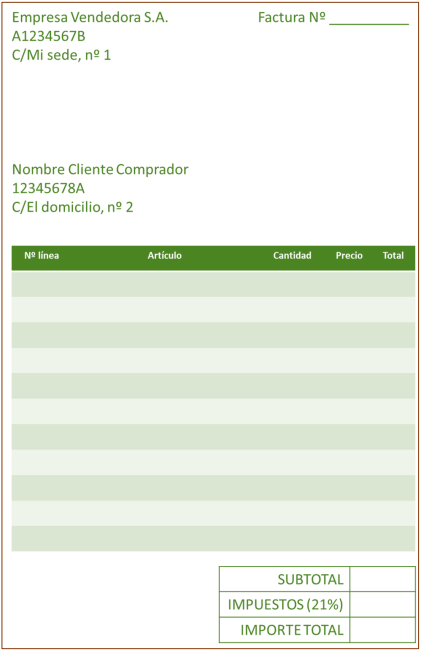
\includegraphics[width=0.5\textwidth]{./Imagenes/Rel1_Ej6.png}
        \caption{Modelo de Factura del Ejercicio~\ref{ej:6}}
        \label{fig:factura}
    \end{figure}

    El Diagrama Entidad-Relación correspondiente se encuentra en la Figura~\ref{fig:ej6}.
    \begin{figure}
        \centering
        \begin{tikzpicture}[node distance=6.3 em]
            \node[entidad] (factura) {Factura};
            \node[relacion] (comprar) [right of=factura] {Comprar} edge(factura);
            \node[relacion] (vender) [left of=factura] {Vender} edge(factura);
            \node[entidad] (cliente) [right of=comprar] {Cliente} edge[Stealth-](comprar);
            \node[entidad] (empresa) [left of=vender] {Empresa} edge[Stealth-](vender);
            \node[relacion] (contiene) [below of=factura] {Contiene} edge(factura);
            \node[entidad] (articulo) [below of=contiene] {Artículo} edge(contiene);

            \node[atributo] (num) [above of=factura] {\key{Número}} edge(factura);
            
            \node[atributo] (nombre) [above of=cliente] {Nombre} edge(cliente);
            \node[atributo] (DNI) [above right of=cliente] {\key{DNI}} edge(cliente);
            \node[atributo] (dir) [below of=cliente, node distance=4em] {Dirección} edge(cliente);

            \node[atributo] (nombre_emp) [above of=empresa] {Nombre} edge(empresa);
            \node[atributo] (CIF) [above left of=empresa] {\key{CIF}} edge(empresa);
            \node[atributo] (dir_emp) [below of=empresa, node distance=4em] {Dirección} edge(empresa);

            \node[atributo] (codigo) [below of=articulo, node distance=4em] {\key{Código}} edge(articulo);
            \node[atributo] (nombre_art) [right of=articulo] {Nombre} edge(articulo);
            \node[atributo] (precio) [left of=articulo] {Precio} edge(articulo);

            \node[atributo] (cantidad) [right of=contiene] {Cantidad} edge(contiene);
        \end{tikzpicture}
        \caption{Diagrama Entidad-Relación del Ejercicio~\ref{ej:6}}
        \label{fig:ej6}
    \end{figure}
\end{ejercicio}

\begin{ejercicio} \label{ej:7}
    En una empresa mecánica se quiere poder calcular el precio de las piezas instaladas en un coche, sabiendo
    que algunas de las piezas pueden tener varios componentes. Para ello debemos representar cada tipo de
    pieza, del que se registra un código y su denominación. Se supone que:
    \begin{itemize}
        \item Hay dos tipos de pieza simple o compuesta.
        \item El precio de un tipo de pieza simple consiste en el valor dicha pieza.
        \item Si el tipo de pieza es compuesto su precio se corresponde con el precio de montaje sin incluir el precio de
        los tipos de pieza que la componen.
        \item Para los tipos de pieza compuestos se registran el número de unidades de cada tipo de pieza que la
        compone.
        \item Un tipo de pieza es componente de un único tipo de pieza compuesta.
    \end{itemize}
    Resuelva el problema considerando:
    \begin{itemize}
        \item Que las piezas compuestas solo pueden estar compuestas de piezas simples.
        
        El Diagrama Entidad-Relación correspondiente se encuentra en la Figura~\ref{fig:ej7_a}.
        \begin{figure}
            \centering
            \begin{tikzpicture}[node distance=6.3 em]
                \node[entidad] (pieza) {Pieza};
                \node[herencia] (tipo) [below of=pieza] {Tipo} edge[participacion obligatoria] node[midway, right] {Disjunta} (pieza);
                \node[entidad] (simple) [below of=tipo, xshift=-8em, yshift=-1em] {Simple} edge(tipo);
                \node[entidad] (compuesta) [below of=tipo, xshift=8em, yshift=-1em] {Compuesta} edge(tipo);
                \node[relacion] (componente) [below of=tipo, yshift=-1em] {Componente} edge[-Stealth](compuesta) edge(simple);

                \node[atributo] (codigo) [left of=pieza] {\key{Código}} edge(pieza);
                \node[atributo] (denominacion) [right of=pieza, node distance=8em] {Denominación} edge(pieza);
                \node[atributo derivado] (precio) [below left of=pieza] {Precio} edge(pieza);

                \node[atributo] (valor) [left of=simple] {Valor} edge(simple);
                \node[atributo] (precio_montaje) [right of=compuesta] {Montaje} edge(compuesta);

                \node[atributo] (unidades) [below of=componente] {Unidades} edge(componente);


            \end{tikzpicture}
            \caption{Diagrama Entidad-Relación del Ejercicio~\ref{ej:7} del apartado 1.}
            \label{fig:ej7_a}
        \end{figure}

        \item Que las piezas compuestas pueden estar compuestas tanto de piezas simples como compuestas.
        
        El Diagrama Entidad-Relación correspondiente se encuentra en la Figura~\ref{fig:ej7_b}.
        \begin{figure}
            \centering
            \begin{tikzpicture}[node distance=6.3 em]
                \node[entidad] (pieza) {Pieza};
                \node[herencia] (tipo) [below of=pieza] {Tipo} edge[participacion obligatoria] node[midway, right] {Disjunta} (pieza);
                \node[entidad] (simple) [below left of=tipo, xshift=-2em, yshift=-1em] {Simple} edge(tipo);
                \node[entidad] (compuesta) [below right of=tipo, xshift=2em, yshift=-1em] {Compuesta} edge(tipo);
                \node[relacion] (componente) [right of=pieza] {Componente} edge[-Stealth](compuesta) edge(pieza);

                \node[atributo] (codigo) [left of=pieza] {\key{Código}} edge(pieza);
                \node[atributo] (denominacion) [above left of=pieza] {Denominación} edge(pieza);
                \node[atributo derivado] (precio) [below left of=pieza] {Precio} edge(pieza);

                \node[atributo] (valor) [left of=simple] {Valor} edge(simple);
                \node[atributo] (precio_montaje) [right of=compuesta] {Montaje} edge(compuesta);

                \node[atributo] (unidades) [right of=componente, xshift=2em] {Unidades} edge(componente);


            \end{tikzpicture}
            \caption{Diagrama Entidad-Relación del Ejercicio~\ref{ej:7} del apartado 2.}
            \label{fig:ej7_b}
        \end{figure}
    \end{itemize}
\end{ejercicio}

\begin{ejercicio} \label{ej:8}
    En una base de datos de una tienda de productos informáticos, los tipos de productos se registran con un
    número de referencia, un fabricante y tienen un precio de venta al público. De los artículos estrella de la tienda
    (impresoras, PCs y portátiles) se registran las siguientes características adicionales:
    \begin{itemize}
        \item Impresoras: color (s/n), resolución (ppp), tipo (láser o inyección de tinta).
        \item PC: procesador, velocidad, RAM, capacidad del disco.
        \item Portátiles: procesador, velocidad, RAM, capacidad del disco, tamaño de pantalla.
    \end{itemize}
    Considere que cada procesador tiene una velocidad determinada.\\

    El Diagrama Entidad-Relación correspondiente se encuentra en la Figura~\ref{fig:ej8}.
    Notemos que, al incluir un procesador como un tipo de producto, que se pueden vender estos también por separado.
    \begin{figure}
        \centering
        \begin{tikzpicture}[node distance=6.3 em]
            \node[entidad] (producto) {Producto};
            \node[relacion] (fabricar) [right of=producto] {Fabricar} edge(producto);
            \node[entidad] (fabricante) [right of=fabricar] {Fabricante} edge[Stealth-](fabricar);

            \node[herencia] (tipo) [below of=producto] {Tipo} edge node[midway, right] {Disjunta} (producto);
            \node[entidad] (impresora) [below left of=tipo, node distance=9 em, xshift=-4em] {Impresora} edge(tipo);
            \node[entidad] (procesador) [below of=tipo] {Procesador} edge(tipo);
            \node[entidad] (ordenador) [below right of=tipo, node distance=9 em, xshift=6em] {Ordenador} edge(tipo);

            \node[herencia] (tipo_pc) [below of=ordenador] {Tipo} edge node[midway, right] {Disjunta} (ordenador);
            \node[entidad] (portatil) [below left of=tipo_pc] {Portátil} edge(tipo_pc);
            \node[entidad] (pc) [below right of=tipo_pc] {PC} edge(tipo_pc);

            \node[atributo] (ref) [left of=producto] {\key{Referencia}} edge(producto);
            \node[atributo] (precio) [below left of=producto, yshift=2em] {PVP} edge(producto);

            \node[atributo] (cod_fab) [right of=fabricante] {\key{Código}} edge(fabricante);
            \node[atributo] (nombre) [below right of=fabricante, yshift=2em] {Nombre} edge(fabricante);

            \node[relacion] (contiene) [right of=procesador] {Contiene} edge[-Stealth](procesador) edge(ordenador);

            \node[atributo] (color) [above of=impresora] {Color} edge(impresora);
            \node[atributo] (resolucion) [above left of=impresora] {Resolución} edge(impresora);
            \node[relacion] (es_tipo) [below of=impresora] {Es} edge(impresora);
            \node[entidad] (tipo_impresora) [left of=es_tipo] {Tipo} edge[Stealth-](es_tipo);
            \node[atributo] (tipo_imp) [below right of=tipo_impresora] {Tipo} edge(tipo_impresora);
            \node[atributo] (cod_tipo) [below of=tipo_impresora] {\key{Código}} edge(tipo_impresora);

            \node[atributo] (velocidad) [below of=procesador] {Velocidad} edge(procesador);
            \node[atributo] (nombre_proc) [below left of=procesador] {Nombre} edge(procesador);

            \node[atributo] (RAM) [above of=ordenador] {RAM} edge(ordenador);
            \node[atributo] (capacidad) [above right of=ordenador] {Capacidad} edge(ordenador);

            \node[atributo] (tam_pantalla) [left of=portatil, xshift=-3em] {Tamaño Pantalla} edge(portatil);
        \end{tikzpicture}
        \caption{Diagrama Entidad-Relación del Ejercicio~\ref{ej:8}}
        \label{fig:ej8}
    \end{figure}
\end{ejercicio}

\begin{ejercicio} \label{ej:9}
    Expresar mediante un diagrama E/R el registro de llamadas entre dos teléfonos, conteniendo fecha y hora de
    inicio y de finalización. Supongamos que un teléfono se identifica mediante un número y que podemos contar
    con dos tipos de teléfono: fijo o móvil. No se contemplan llamadas en las que participen más de dos teléfonos.

    El Diagrama Entidad-Relación correspondiente se encuentra en la Figura~\ref{fig:ej9}.
    \begin{figure}
        \centering
        \begin{tikzpicture}[node distance=6.3 em]
            \node[entidad] (telefono) {Teléfono};
            \node[herencia] (tipo) [below of=telefono] {Tipo} edge[participacion obligatoria] node[midway, left] {Disjunta} (telefono);
            \node[entidad] (fijo) [below left of=tipo, xshift=-2em] {Fijo} edge(tipo);
            \node[entidad] (movil) [below right of=tipo, xshift=2em] {Móvil} edge(tipo);
            
            \node[relacion] (llamada) [right of=telefono, node distance=10em] {Llamada};
            \draw[Stealth-] (telefono.north east) |- node[near end, above] {Llama} (llamada.north);
            \draw[Stealth-] (telefono.south east) |- node[near end, below] {Es llamado por} (llamada.south);

            \node[atributo] (num) [left of=telefono] {\key{Número}} edge(telefono);

            \node[atributo] (fecha_ini) [right of=llamada, node distance=7em] {\key{Fecha Inicio}} edge[union discriminante](llamada);
            \node[atributo] (fecha_fin) [below right of=llamada] {Fecha Fin} edge(llamada);
        \end{tikzpicture}
        \caption{Diagrama Entidad-Relación del Ejercicio~\ref{ej:9}}
        \label{fig:ej9}
    \end{figure}
\end{ejercicio}

\begin{ejercicio} \label{ej:10}
    Una receta de cocina se describe mediante una serie de ingredientes y de pasos de ejecución. En cada paso
    de ejecución se describe una acción y se utilizan una serie de ingredientes. Las recetas se caracterizan por:
    \begin{itemize}
        \item Código; Nombre; Tipo (primero, segundo y postre) y dificultad (alta, media, baja).
        \item A su vez, los ingredientes se caracterizan por: Código; Nombre: Tipo (grano, polvo, troceado y otro) y precio.
    \end{itemize}

    El Diagrama Entidad-Relación correspondiente se encuentra en la Figura~\ref{fig:ej10}.
    Notemos que ambas jerarquías descritas podrían añadirse simplemente como un atributo más.
    \begin{figure}
        \centering
        \begin{tikzpicture}[node distance=7 em]
            \node[entidad] (receta) {Receta};
            \node[herencia] (tipo) [below of=receta] {Tipo} edge[participacion obligatoria] node[midway, right] {Disjunta} (receta);
            \node[entidad] (primero) [below left of=tipo, xshift=-2em] {Primero} edge(tipo);
            \node[entidad] (segundo) [below of=tipo] {Segundo} edge(tipo);
            \node[entidad] (postre) [below right of=tipo, xshift=2em] {Postre} edge(tipo);

            \node[entidad debil] (paso) [right of=receta] {Paso} edge(receta);
            \node[relacion] (utiliza) [right of=paso] {Utiliza} edge(paso);
            \node[entidad] (ingrediente) [right of=utiliza] {Ingrediente} edge(utiliza);

            \node[herencia] (tipo_ing) [below of=ingrediente] {Tipo} edge node[midway, left] {Disjunta} (ingrediente);
            \node[entidad] (grano) [below left of=tipo_ing, xshift=-2em] {Grano} edge(tipo_ing);
            \node[entidad] (polvo) [below of=tipo_ing] {Polvo} edge(tipo_ing);
            \node[entidad] (troceado) [below right of=tipo_ing, xshift=2em] {Troceado} edge(tipo_ing);

            \node[atributo] (codigo_rec) [above left of=receta, yshift=-1em] {\key{Código}} edge(receta);
            \node[atributo] (nombre) [left of=receta] {Nombre} edge(receta);
            \node[atributo] (dificultad) [below left of=receta, yshift=1em] {Dificultad} edge(receta);

            \node[atributo] (codigo_ing) [right of=ingrediente] {\key{Código}} edge(ingrediente);
            \node[atributo] (nombre_ing) [above right of=ingrediente, yshift=-1em] {Nombre} edge(ingrediente);
            \node[atributo] (precio) [below right of=ingrediente, yshift=1em] {Precio} edge(ingrediente);

            \node[atributo] (nombre_paso) [below of=paso] {Nombre} edge(paso);
            \node[atributo] (accion) [below right of=paso] {Acción} edge(paso);

            \node[atributo] (cantidad) [above of=utiliza] {Cantidad} edge(utiliza);
            \node[atributo] (orden) [above of=paso] {\key{Orden}} edge[union discriminante] (paso);


        \end{tikzpicture}
        \caption{Diagrama Entidad-Relación del Ejercicio~\ref{ej:10}}
        \label{fig:ej10}
    \end{figure}
\end{ejercicio}

\begin{ejercicio} \label{ej:11}
    Se trata de modelar la programación que ofrecen los canales de TV. La información que se desea almacenar
    es la siguiente:
    \begin{itemize}
        \item Presentador (DNI, Nombre, Especialidad).
        \item Canales (Nombre, Empresa, Tipo).
        \item Programas (Código, Nombre, Duración, Tipo).
    \end{itemize}
    Las restricciones de integridad que deben mantenerse son las siguientes:
    \begin{itemize}
        \item Existen tres tipos de programas:
        \begin{itemize}
            \item Películas, de las que hay que conocer Título, Tema y Año.
            \item Concursos.
            \item Informativos.
        \end{itemize}
        \item En cada momento, solo hay un programa en emisión en cada canal.
        \item Los concursos solo pueden ser presentados por un presentador, pero un presentador puede serlo de varios concursos.
        \item Los informativos pueden ser presentados por varios presentadores y un presentador puede serlo de varios también.
    \end{itemize}

    El Diagrama Entidad-Relación correspondiente se encuentra en la Figura~\ref{fig:ej11}.
    Respecto a la condición de que solo haya un programa en emisión en cada canal, se ha añadido el atributo \emph{Fecha} en la relación \emph{Emite}.
    Esto provoca que, en un canal, dos programas no puedan comenzar a emitirse en la misma fecha, aunque no evita que, debido a la duración, se solapen.
    Esto último habrá que controlarlo en la programación.
    \begin{figure}
        \centering
        \begin{tikzpicture}[node distance=6.3 em]
            \node[entidad] (programa) {Programa};
            \node[herencia] (tipo) [below of=programa] {Es un} edge[participacion obligatoria] node[midway, right] {Disjunta} (programa);
            \node[entidad] (pelicula) [below left of=tipo, xshift=-2em, yshift=-1.8em] {Película} edge(tipo);
            \node[entidad] (concurso) [below of=tipo] {Concurso} edge(tipo);
            \node[entidad] (informativo) [below right of=tipo, xshift=2em, yshift=-1.8em] {Informativo} edge(tipo);

            \node[relacion] (emite) [right of=programa] {Emite} edge(programa);
            \node[entidad] (canal) [right of=emite] {Canal} edge(emite);

            \node[relacion] (presenta_informativo) [right of=informativo] {Informa} edge(informativo);
            \node[entidad] (presentador) [below of=presenta_informativo] {Presentador} edge(presenta_informativo);

            \node[relacion] (presenta_concurso) [below of=concurso] {Presenta} edge(concurso) edge[-Stealth](presentador);

            \node[atributo] (DNI) [right of=presentador] {\key{DNI}} edge(presentador);
            \node[atributo] (nombre) [above right of=presentador] {Nombre} edge(presentador);
            \node[atributo] (especialidad) [below right of=presentador] {Especialidad} edge(presentador);

            \node[atributo] (nombre_canal) [above right of=canal] {\key{Nombre}} edge(canal);
            \node[atributo] (empresa) [right of=canal] {Empresa} edge(canal);
            \node[atributo] (tipo_canal) [below right of=canal] {Tipo} edge(canal);

            \node[atributo] (codigo) [left of=programa] {\key{Código}} edge(programa);
            \node[atributo] (nombre_prog) [above left of=programa] {Nombre} edge(programa);
            \node[atributo] (duracion) [above of=programa] {Duración} edge(programa);
            \node[atributo] (tipo_prog) [above right of=programa] {Tipo} edge(programa);

            \node[atributo] (titulo) [above of=pelicula] {\key{Título}} edge(pelicula);
            \node[atributo] (tema) [below of=pelicula] {Tema} edge(pelicula);
            \node[atributo] (año) [below left of=pelicula] {Año} edge(pelicula);

            \node[atributo] (fecha_emision) [below of=emite] {\key{Fecha}} edge[union discriminante](emite);
        \end{tikzpicture}
        \caption{Diagrama Entidad-Relación del Ejercicio~\ref{ej:11}}
        \label{fig:ej11}
    \end{figure}
\end{ejercicio}

\begin{ejercicio} \label{ej:12}
    Diseña una BD que gestione los datos que se manejan en las comisarías de policía de una ciudad. En dicha BD
    debe registrarse la siguiente información:
    \begin{itemize}
        \item DELINCUENTES, que van identificados por su DNI y de los que debe conocerse Nombre y Apellidos, Fecha
        de Nacimiento, Domicilio y Nacionalidad.
        \item DELITOS, identificados por un código y de los que hay que registrar su Nombre, Tipo, y Penas Máxima y
        Mínima.
        \item AGENTES, identificados por su Número de Placa y de los que debe conocerse su DNI, Nombre y Apellidos,
        Domicilio y Fecha de Ingreso en el cuerpo.
        \item COMISARÍAS, identificadas por un Nombre y de las que debe registrarse su Localización.
    \end{itemize}
    Las restricciones semánticas que deben cumplirse son las siguientes:
    \begin{itemize}
        \item Existen dos tipos de AGENTES: OFICIALES y POLICIAS.
        \item De los oficiales debe conocerse la Especialización y los años de Experiencia.
        \item Un oficial es responsable de un grupo de policías y un policía solo depende de un oficial.
        \item Cada comisaría la dirige un oficial.
        \item Cuando un delincuente es detenido, debe registrarse el lugar, la fecha y la hora de la detención y qué
        agentes han participado en la misma.
        \item De los delitos cometidos, debe conocerse el lugar, la fecha y la hora, así como los delincuentes que han
        participado.
    \end{itemize}

    El Diagrama Entidad-Relación correspondiente se encuentra en la Figura~\ref{fig:ej12}. Algunas consideraciones son:
    \begin{itemize}
        \item Se ha establecido la superclase \emph{Persona} para \emph{Agente} y \emph{Delincuente}, ya que comparten varios atributos.
        Además, en el hipotético caso de que un agente sea detenido, no habría redundancia.
        \item La relación \emph{Realiza} tiene cardinalidad $M:N$, ya que una comisión de un delito puede ser realizada por varios delincuentes, y un delincuente puede realizar varias comisiones de delito en su vida.
        \item La relación \emph{Es} tiene cardinalidad $M:N$, ya que una comisión de delito puede ser de varios tipos (por ejemplo, en un atraco, puede haber robo, secuestro, allanamiento de morada, etc.), y un tipo de delito puede ser cometido en varias ocasiones.
        \item En un primer momento, podríamos haber establecido \emph{Detención} como una relación entre \emph{Agente} y \emph{Delincuente}, pero los atributos asociados a la detención (lugar, fecha y hora) se repitirían en gran cantidad de ocasiones (si $n$ agentes participan en la misma detención, se repetirían $n$ veces).
        Por ello, se ha decidido crear una entidad propia para la detención.
        \item De igual forma, la comisión de un delito se ha considerado como una entidad propia, ya que, si no, si $n$ delincuentes realizan el mismo delito, se repetirían $n$ veces los atributos asociados a la comisión del delito.
    \end{itemize}
    \begin{figure}
        \centering
        \begin{tikzpicture}[node distance=6.3 em]

            \node[entidad] (persona) {Persona};
            \node[herencia] (tipo_persona) [below of=persona] {Tipo} edge[participacion obligatoria] (persona);

            \node[entidad] (agente) [below left of=tipo_persona, xshift=-6.5em, yshift=-2em] {Agente} edge(tipo_persona);
            \node[herencia] (tipo) [below of=agente] {Tipo} edge[participacion obligatoria] node[midway, right] {Disjunta} (agente);
            \node[entidad] (oficial) [below right of=tipo, xshift=2em] {Oficial} edge(tipo);
            \node[entidad] (policia) [below left of=tipo, xshift=-2em] {Policía} edge(tipo);

            \node[relacion] (responsable) [below of=tipo, yshift=-2em] {Responsable} edge[-Stealth](oficial) edge(policia);
            \node[relacion] (dirige) [below of=oficial, node distance=5.5em] {Dirige} edge[-Stealth](oficial);
            \node[entidad] (comisaria) [below of=dirige, node distance=5.5em] {Comisaría} edge[Stealth-](dirige);

            \node[relacion] (participa) [right of=agente, node distance=5.5em] {Participa} edge(agente);
            \node[entidad] (detencion) [right of=participa, node distance=5.5em] {Detención} edge(participa);
            \node[relacion] (sufre) [right of=detencion, node distance=5.5em] {Sufre} edge(detencion);
            \node[entidad] (delincuente) [right of=sufre, node distance=5.5em] {Delincuente} edge(sufre) edge(tipo_persona);

            \node[relacion] (realiza) [below of=delincuente] {Realiza} edge(delincuente);
            \node[entidad] (comision_deltito) [below of=realiza, align=center] {Comisión\\Delito} edge(realiza);

            \node[relacion] (es) [below of=comision_deltito, node distance=5.5em] {Es} edge(comision_deltito);
            \node[entidad] (delito) [below of=es, node distance=5.5em] {Delito} edge(es);

            \node[atributo] (DNI) [right of=persona] {\key{DNI}} edge(persona);
            \node[atributo] (nombre) [below right of=persona, yshift=2em] {Nombre} edge(persona);
            \node[atributo] (apellidos) [left of=persona] {Apellidos} edge(persona);
            \node[atributo] (fecha_nac_delincuentes) [above of=delincuente] {Fecha Nacimiento} edge(delincuente);
            \node[atributo] (domicilio) [below left of=persona, yshift=2em] {Domicilio} edge(persona);
            \node[atributo] (nacionalidad_delincuentes) [above right of=delincuente] {Nacionalidad} edge(delincuente);

            \node[atributo] (codigo_delito) [above left of=delito] {\key{Código}} edge(delito);
            \node[atributo] (nombre_delito) [above right of=delito] {Nombre} edge(delito);
            \node[atributo] (tipo_delito) [right of=delito] {Tipo} edge(delito);
            \node[atributo] (pena_max) [left of=delito, yshift=2em, node distance=7em] {Pena Máxima} edge(delito);
            \node[atributo] (pena_min) [left of=delito, node distance=7em] {Pena Mínima} edge(delito);

            \node[atributo] (num_placa) [above of=agente] {\key{Número Placa}} edge(agente);
            \node[atributo] (fecha_ingreso) [above left of=agente] {Fecha Ingreso} edge(agente);

            \node[atributo] (nombre_comisaria) [above left of=comisaria, yshift=-2em] {\key{Nombre}} edge(comisaria);
            \node[atributo] (localizacion) [left of=comisaria, node distance=7.2em] {Localización} edge(comisaria);

            \node[atributo] (especializacion) [below right of=oficial, xshift=1em, yshift=2em] {Especialización} edge(oficial);
            \node[atributo] (fecha_ascenso) [right of=oficial, node distance=7em] {Fecha Ascenso} edge(oficial);

            \node[atributo] (codigo_detencion) [below right of=detencion] {\key{Código}} edge(detencion);
            \node[atributo] (lugar_detencion) [below of=detencion] {Lugar} edge(detencion);
            \node[atributo] (fecha_detencion) [below left of=detencion] {Fecha} edge(detencion);

            \node[atributo] (lugar_comision) [above right of=comision_deltito, yshift=-2em] {Lugar} edge(comision_deltito);
            \node[atributo] (fecha_comision) [below right of=comision_deltito, yshift=2em] {Fecha} edge(comision_deltito);
            \node[atributo] (codigo_comision) [right of=comision_deltito] {\key{Código}} edge(comision_deltito);
        \end{tikzpicture}
        \caption{Diagrama Entidad-Relación del Ejercicio~\ref{ej:12}}
        \label{fig:ej12}
    \end{figure}
\end{ejercicio}

\begin{ejercicio} \label{ej:13}
    Queremos gestionar una base de datos que contenga información sobre objetos astronómicos:
    \begin{itemize}
        \item Un objeto astronómico se identifica mediante un código y, además, se registra la fecha y observatorio
        donde se hizo su descubrimiento.
        \item Los objetos astronómicos los vamos a clasificar en:
        \begin{itemize}
            \item Objetos de baja emisión de luz: Planetas y Satélites.
            \item Objetos de alta emisión de luz: Estrellas.
        \end{itemize}
        \item De los planetas almacenamos el tipo de planeta.
        \item De los satélites nos interesa saber el tipo de satélite.
        \item De las estrellas almacenamos el tipo y subtipo al que pertenecen.
        \item Además, queremos describir el hecho de que:
        \begin{itemize}
            \item Un satélite gira alrededor de un planeta, conociéndose la distancia entre ellos, y también
            almacenamos a cuantos años luz se encuentran entre sí. Alrededor de un planeta pueden girar
            diferentes satélites.
            \item Un planeta, junto con sus satélites, giran alrededor de una estrella. También se almacena a
            cuantos años luz distan entre sí. Alrededor de una estrella pueden girar diferentes planetas.
            \item Un grupo de estrellas forman una constelación y cada estrella puede estar en varias
            constelaciones.
            \item De las constelaciones nos interesa almacenar el código y nombre.
        \end{itemize}
    \end{itemize}

    El Diagrama Entidad-Relación correspondiente se encuentra en la Figura~\ref{fig:ej13}.
    Notemos que hemos supuesto que, además de planetas y satélites, también se pueden descubrir otros objetos astronómicos de baja emisión de luz.
    \begin{figure}
        \centering
        \begin{tikzpicture}[node distance=6.3 em]
            \node[entidad] (objeto) {Objeto Astronómico};
            \node[relacion] (descubrimiento) [right of=objeto, node distance=10em] {Descubrimiento} edge(objeto);
            \node[entidad] (observatorio) [right of=descubrimiento, node distance=8em] {Observatorio} edge[Stealth-](descubrimiento);
            \node[atributo] (fecha_desc) [below of=descubrimiento] {Fecha} edge(descubrimiento);

            \node[herencia] (tipo) [below of=objeto] {Tipo} edge[participacion obligatoria] node[midway, right] {Disjunta} (objeto);
            \node[entidad] (baja_emision) [below left of=tipo, xshift=-4em] {Baja Emisión} edge(tipo);
            \node[entidad] (alta_emision) [below right of=tipo, xshift=4em, align=center] {Alta Emisión} edge(tipo);
            
            \node[herencia] (tipo_baja) [below of=baja_emision] {Tipo} edge node[midway, right] {Disjunta} (baja_emision);
            \node[entidad] (planeta) [below right of=tipo_baja] {Planeta} edge(tipo_baja);
            \node[entidad] (satelite) [below left of=tipo_baja] {Satélite} edge(tipo_baja);

            \node[herencia] (tipo_alta) [below of=alta_emision] {Tipo} edge node[midway, right] {Disjunta} (alta_emision);
            \node[entidad] (estrella) [below of=tipo_alta] {Estrella} edge(tipo_alta);

            \node[relacion] (gira_satelite) [below right of=satelite] {Gira} edge(satelite) edge[-Stealth](planeta);
            \node[atributo] (distancia) [below of=gira_satelite, yshift=2.5em] {Distancia} edge(gira_satelite);

            \node[relacion] (gira_planeta) [above right of=planeta] {Orbita} edge(planeta) edge[-Stealth](estrella);
            \node[atributo] (dist_planeta) [above of=gira_planeta, node distance=5em] {Distancia} edge(gira_planeta);

            \node[atributo] (cod_objeto) [left of=objeto, node distance=8em] {\key{Código}} edge(objeto);

            \node[atributo] (tipo_planeta) [below of=planeta] {Tipo} edge(planeta);
            \node[atributo] (tipo_satelite) [below of=satelite] {Tipo} edge(satelite);
            \node[relacion] (es) [right of=estrella, node distance=7em] {Es} edge(estrella);
            \node[entidad] (subtipo_estrella) [above of=es, node distance=5em] {Subtipo} edge[Stealth-](es);
            \node[atributo] (cod_subtipo) [right of=subtipo_estrella, yshift=2em] {\key{Código}} edge(subtipo_estrella);
            \node[atributo] (nombre_subtipo) [right of=subtipo_estrella, yshift=-2em] {Nombre} edge(subtipo_estrella);
            \node[relacion] (es_tipo) [above of=subtipo_estrella, node distance=5em] {Es} edge(subtipo_estrella);
            \node[entidad] (tipo_estrella) [above of=es_tipo, node distance=5em] {Tipo} edge[Stealth-](es_tipo);
            \node[atributo] (cod_tipo) [right of=tipo_estrella, yshift=2em] {\key{Código}} edge(tipo_estrella);
            \node[atributo] (nombre_tipo) [right of=tipo_estrella, yshift=-2em] {Nombre} edge(tipo_estrella);


            \node[relacion] (forman) [left of=estrella] {Forman} edge(estrella);
            \node[entidad] (constelacion) [below of=forman] {Constelación} edge(forman);
            \node[atributo] (nombre_const) [right of=constelacion] {Nombre} edge(constelacion);
            \node[atributo] (cod_const) [above right of=constelacion, yshift=-2em] {\key{Código}} edge(constelacion);

        \end{tikzpicture}
        \caption{Diagrama Entidad-Relación del Ejercicio~\ref{ej:13}}
        \label{fig:ej13}
    \end{figure}
\end{ejercicio}

\begin{ejercicio} \label{ej:14}
    En una base de datos de un hospital hay información relativa a pacientes (de los que se almacena el DNI,
    nombre, dirección y teléfono) e historias clínicas (que tienen un código y una fecha de creación). Cada
    persona tiene una única historia clínica y cada historia clínica corresponde a una sola persona. Una historia
    clínica consta de distintos episodios o ingresos que se van numerando de forma consecutiva y de los cuales
    se registra además el motivo del episodio y la fecha en la que se produce.

    El diagrama Entidad-Relación correspondiente se encuentra en la Figura~\ref{fig:ej14}.
    Notemos que establecer la participación obligatoria de la relación \emph{Tiene} en la entidad \emph{Historia Clínica} podría ser válida.
    \begin{figure}
        \centering
        \begin{tikzpicture}[node distance=7.3 em]
            \node[entidad] (paciente) {Paciente};
            \node[relacion] (tiene) [right of=paciente] {Tiene} edge[-Stealth](paciente);
            \node[entidad] (historia) [right of=tiene] {Historia Clínica} edge[Stealth-](tiene);
            \node[entidad debil] (ingreso) [right of=historia] {Ingreso} edge(historia);

            \node[atributo] (DNI) [above left of=paciente, yshift=-2em] {\key{DNI}} edge(paciente);
            \node[atributo] (nombre) [above of=paciente, node distance=4 em] {Nombre} edge(paciente);
            \node[atributo] (direccion) [below left of=paciente, yshift=2em] {Dirección} edge(paciente);
            \node[atributo] (telefono) [below of=paciente, node distance=4 em] {Teléfono} edge(paciente);

            \node[atributo] (codigo) [above of=historia, node distance=4 em] {\key{Código}} edge(historia);
            \node[atributo] (fecha_creacion) [below of=historia, node distance=4 em] {Fecha Creación} edge(historia);

            \node[atributo] (numero) [above of=ingreso, node distance=4 em] {\key{Número}} edge[union discriminante](ingreso);
            \node[atributo] (motivo) [below of=ingreso, node distance=4 em] {Motivo} edge(ingreso);
            \node[atributo] (fecha_ingreso) [right of=ingreso] {Fecha Ingreso} edge(ingreso);
        \end{tikzpicture}
        \caption{Diagrama Entidad-Relación del Ejercicio~\ref{ej:14}}
        \label{fig:ej14}
    \end{figure}
\end{ejercicio}

\begin{ejercicio} \label{ej:15}
    En una base de datos hay información relativa a empleados (sobre los que se conoce el identificador, nombre
    y dirección). Hay dos tipos de empleados: fijos y eventuales. De los fijos se conoce la fecha de inicio del
    contrato y la fecha de la última revisión salarial. De los eventuales, se conoce la fecha de contratación y la
    duración del contrato. En la empresa hay una serie de tareas (código y descripción). Determinadas tareas
    solo pueden hacerlas empleados fijos.

    El diagrama Entidad-Relación correspondiente se encuentra en la Figura~\ref{fig:ej15}.
    \begin{figure}
        \centering
        \begin{tikzpicture}[node distance=5 em]
            \node[entidad] (empleado) {Empleado};
            \node[herencia] (tipo) [below of=empleado] {Tipo} edge[participacion obligatoria] node[midway, right] {Disjunta} (empleado);
            \node[entidad] (fijo) [below left of=tipo, xshift=-4em] {Fijo} edge(tipo);
            \node[entidad] (eventual) [below right of=tipo, xshift=4em] {Eventual} edge(tipo);

            \node[relacion] (fijo_realiza) [below of=fijo, align=center] {Fijo\\Realiza} edge(fijo);
            \node[entidad] (tarea) [below of=tipo, yshift=-3.5em] {Tarea} edge(fijo_realiza);
            \node[herencia] (tipo_tarea) [below of=tarea] {Tipo} edge[participacion obligatoria] node[midway, right] {Disjunta} (tarea);
            \node[entidad] (específica) [below left of=tipo_tarea, xshift=-4em] {Específica} edge(tipo_tarea);
            \node[entidad] (general) [below right of=tipo_tarea, xshift=4em] {General} edge(tipo_tarea);

            \node[relacion] (eventual_realiza) [below of=eventual, align=center] {Eventual\\Realiza} edge(eventual) edge(general);

            \node[atributo] (identificador) [above left of=empleado] {\key{Identificador}} edge(empleado);
            \node[atributo] (nombre) [right of=empleado, xshift=2em] {Nombre} edge(empleado);
            \node[atributo] (direccion) [above right of=empleado] {Dirección} edge(empleado);
            \node[atributo] (fecha_contratacion) [left of=empleado, xshift=-4em] {Fecha Contratación} edge(empleado);

            \node[atributo] (fecha_rev) [above left of=fijo] {Fecha Última Revisión} edge(fijo);
            \node[atributo] (duracion) [above of=eventual] {Duración} edge(eventual);
        \end{tikzpicture}
        \caption{Diagrama Entidad-Relación del Ejercicio~\ref{ej:15}}
        \label{fig:ej15}
    \end{figure}
\end{ejercicio}

\begin{ejercicio} \label{ej:16}
    En una base de datos hay información sobre proveedores (de los que se almacena el código de proveedor,
    nombre y dirección) y productos (de los que se almacena código del producto, nombre, precio y descripción).
    En general los proveedores suministran varios productos. Un producto puede ser suministrado por más de un
    proveedor. ¿Cómo cambia el diseño si se quiere registrar el precio al que cada proveedor suministra el
    producto?
    
    El Diagrama Entidad-Relación correspondiente se encuentra en la Figura~\ref{fig:ej16}.
    Notemos que, en el caso de que se quiera registrar el precio al que cada proveedor suministra el producto, el atributo \emph{Precio} debería ser parte de la relación \emph{Suministra}, sin ser discriminante.
    \begin{figure}
        \centering
        \begin{tikzpicture}[node distance=7 em]
            \node[entidad] (proveedor) {Proveedor};
            \node[relacion] (suministra) [right of=proveedor] {Suministra} edge(proveedor);
            \node[entidad] (producto) [right of=suministra] {Producto} edge (suministra);

            \node[atributo] (codigo_prov) [above left of=proveedor, yshift=-2em] {\key{Código}} edge(proveedor);
            \node[atributo] (nombre_prov) [above of=proveedor, node distance=4 em] {Nombre} edge(proveedor);
            \node[atributo] (direccion_prov) [below left of=proveedor, yshift=2em] {Dirección} edge(proveedor);

            \node[atributo] (codigo_prod) [above of=producto, node distance=4 em] {\key{Código}} edge(producto);
            \node[atributo] (nombre_prod) [below of=producto, node distance=4 em] {Nombre} edge(producto);
            \node[atributo] (precio) [right of=producto] {Precio} edge(producto);
            \node[atributo] (descripcion) [above right of=producto, node distance=4 em, xshift=3em] {Descripción} edge(producto);
        \end{tikzpicture}
        \caption{Diagrama Entidad-Relación del Ejercicio~\ref{ej:16}}
        \label{fig:ej16}
    \end{figure}
\end{ejercicio}


\begin{ejercicio} \label{ej:17}
    En la base de datos hay información sobre el contenido de distintos libros de texto. Hay información relativa
    a los libros (de los que se almacena el ISBN, título y editorial) y de los capítulos de cada libro (que tienen un
    número de capítulo y un título de capítulo).
    
    El Diagrama Entidad-Relación correspondiente se encuentra en la Figura~\ref{fig:ej17}.
    \begin{figure}
        \centering
        \begin{tikzpicture}[node distance=6.3 em]
            \node[entidad] (libro) {Libro};
            \node[entidad debil] (capitulo) [right of=libro, node distance=9em] {Capítulo} edge(libro);

            \node[atributo] (ISBN) [above left of=libro] {\key{ISBN}} edge(libro);
            \node[atributo] (titulo) [above of=libro, node distance=4 em] {Título} edge(libro);
            \node[atributo] (editorial) [left of=libro] {Editorial} edge(libro);

            \node[atributo] (num_cap) [above of=capitulo, node distance=4 em] {\key{Número}} edge[union discriminante](capitulo);
            \node[atributo] (titulo_cap) [right of=capitulo] {Título} edge(capitulo);
        \end{tikzpicture}
        \caption{Diagrama Entidad-Relación del Ejercicio~\ref{ej:17}}
        \label{fig:ej17}
    \end{figure}
\end{ejercicio}

\begin{ejercicio} \label{ej:18}
    Se desea diseñar una base de datos de restaurantes de la provincia de Granada. La información que se desea
    almacenar es la siguiente:
    \begin{itemize}
        \item De cada restaurante, almacenaremos nombre, CIF, domicilio. No hay dos restaurantes con el mismo
        nombre.
        \item Cada restaurante tiene unas personas propietarias (caracterizadas por su DNI, nombre y domicilio).
        \item De cada restaurante se desea registrar el horario de apertura, con la idea de poder facilitar luego
        información sobre qué restaurantes están abiertos en un momento dado.
        \item En cada restaurante trabaja un conjunto de empleados (nombre, DNI, domicilio). También se
        almacena el tipo de trabajo que desempeña el empleado en el restaurante, que puede variar de un
        restaurante a otro. Los propietarios de un restaurante también pueden ser empleados del mismo o
        de otro restaurante.
    \end{itemize}

    El Diagrama Entidad-Relación correspondiente se encuentra en la Figura~\ref{fig:ej18}.
    Notemos que:
    \begin{itemize}
        \item No establecemos una relación de jerarquía, ya que el saber si alguien es propietario o empleado viene determinada por participar o no en cada relación.
        \item Hemos establecido el atributo \emph{Tipo} como discrminante, ya que suponemos que un empleado puede trabajar en un restaurante varias veces con distintos trabajos.
        \item Respecto a los horarios, para poder consultar, por ejemplo, todos los restaurantes que abren un festivo a las $17h$,
        hemos establecido una entidad débil \emph{Tramo}, que representa cada tramo horario de apertura del restaurante. Mediante programación tendríamos que controlar que no se solapasen.
    \end{itemize}
    \begin{figure}
        \centering
        \begin{tikzpicture}[node distance=6.3 em]
            \node[entidad] (persona) {Persona};

            \node[relacion] (posee) [above right of=persona, xshift=6em] {Posee} edge(persona);
            \node[relacion] (trabaja) [below right of=persona, xshift=6em] {Trabaja} edge(persona);


            \node[entidad] (restaurante) [above right of=trabaja, xshift=6em] {Restaurante} edge(posee) edge(trabaja);
            \node[atributo] (nombre_rest) [above of=restaurante, yshift=-2em] {\key{Nombre}} edge(restaurante);
            \node[atributo] (CIF) [above right of=restaurante] {\key{CIF}} edge(restaurante);
            \node[atributo] (domicilio_rest) [right of=restaurante] {Domicilio} edge(restaurante);

            \node[atributo] (tipo_trabajo) [left of=trabaja] {\key{Tipo}} edge[union discriminante](trabaja);

            \node[atributo] (nombre) [above of=persona, xshift=-5em, node distance=5em] {Nombre} edge(persona);
            \node[atributo] (DNI) [above of=persona, node distance=5em] {\key{DNI}} edge(persona);
            \node[atributo] (domicilio) [left of=persona] {Domicilio} edge(persona);

            \node[entidad debil] (tramo) [below of=restaurante, node distance=4em] {Tramo} edge(restaurante);
            \node[atributo] (cod_tramo) [below left of=tramo, xshift=-2em] {\key{Código}} edge[union discriminante](tramo);
            \node[atributo] (hora_inicio) [below right of=tramo, xshift=2em] {Hora Inicio} edge(tramo);
            \node[atributo] (hora_fin) [right of=tramo] {Hora Fin} edge(tramo);
            \node[atributo] (tipo_dia) [below of=tramo, node distance=4em] {Tipo Día} edge(tramo);
        \end{tikzpicture}
        \caption{Diagrama Entidad-Relación del Ejercicio~\ref{ej:18}}
        \label{fig:ej18}
    \end{figure}
\end{ejercicio}

\begin{ejercicio} \label{ej:19}
    Se desea elaborar una base de datos para almacenar datos de promociones inmobiliarias.
    \begin{itemize}
        \item De una promoción deseamos registrar su municipio, la dirección y el tipo de promoción (si es libre o
        de protección oficial).
        \item Una promoción se compone de una serie de viviendas que van numeradas y tienen un plano asociado.
        \item Las promociones tienen promotores. Hay dos tipos de promotores: privados (de los que se desea saber
        su NIF, nombre y años de experiencia) o públicos (de los que se desea saber su, NIF, nombre y ámbito
        -municipal, autonómico, nacional). Los promotores públicos solo pueden llevar promociones de
        protección oficial.
        \item Asimismo, una promoción tiene asociado uno o varios constructores, de los que se desea registrar el
        NIF, el nombre y el tamaño de la empresa.
    \end{itemize}

    El Diagrama Entidad-Relación correspondiente se encuentra en la Figura~\ref{fig:ej19}.
    \begin{figure}
        \centering
        \begin{tikzpicture}[node distance=6.3 em]
            \node[entidad] (persona) {Persona};
            \node[herencia] (tipo_persona) [below of=persona, yshift=2em] {Tipo} edge(persona);
            \node[entidad] (promotor) [below right of=tipo_persona] {Promotor} edge(tipo_persona);
            \node[entidad] (constructor) [below left of=tipo_persona] {Constructor} edge(tipo_persona);

            \node[relacion] (asociado) [left of=constructor] {Asociado} edge(constructor);
            \node[entidad] (promocion) [below of=asociado] {Promoción} edge(asociado);

            \node[entidad debil] (vivienda) [above left of=promocion, xshift=-2em] {Vivienda} edge(promocion);
            
            \node[herencia] (tipo_promocion) [below of=promocion] {Tipo} edge[participacion obligatoria] node[midway, right] {Disjunta} (promocion);
            \node[entidad] (libre) [below left of=tipo_promocion] {Libre} edge(tipo_promocion);
            \node[entidad] (proteccion) [below right of=tipo_promocion] {Protección Oficial} edge(tipo_promocion);

            \node[herencia] (tipo_promotor) [below of=promotor] {Tipo} edge[participacion obligatoria] node[midway, right] {Disjunta} (promotor);
            \node[entidad] (privado) [below left of=tipo_promotor] {Privado} edge(tipo_promotor);
            \node[entidad] (publico) [below right of=tipo_promotor] {Público} edge(tipo_promotor);

            \node[relacion] (encargarse_privado) [above left of=privado, align=center, xshift=1.2em] {Encargarse\\Privado} edge(privado) edge(promocion);
            \node[relacion] (encargarse_publico) [below of=publico, align=center] {Encargarse\\Público} edge(publico) edge(proteccion);

            \node[atributo] (NIF) [left of=persona] {\key{NIF}} edge(persona);
            \node[atributo] (nombre) [right of=persona] {Nombre} edge(persona);

            \node[atributo] (cod_promocion) [left of=promocion] {\key{Código}} edge(promocion);
            \node[atributo] (municipio) [below left of=promocion, yshift=2.2em, xshift=-2em] {Municipio} edge(promocion);
            \node[atributo] (direccion) [below left of=promocion, yshift=0.1em] {Dirección} edge(promocion);

            \node[atributo] (numero) [above left of=vivienda] {\key{Número}} edge[union discriminante](vivienda);
            \node[atributo] (plano) [above of=vivienda] {Plano} edge(vivienda);

            \node[atributo] (años_exp) [below of=privado, node distance=3em] {Años Experiencia} edge(privado);
            \node[atributo] (ambito) [above of=publico, node distance=3em] {Ámbito} edge(publico);

            \node[atributo] (tamaño) [above left of=constructor, node distance=4em] {Tamaño} edge(constructor);
        \end{tikzpicture}
        \caption{Diagrama Entidad-Relación del Ejercicio~\ref{ej:19}}
        \label{fig:ej19}
    \end{figure}
\end{ejercicio}

\begin{ejercicio} \label{ej:20}
    Un estudio de arquitectura pretende diseñar una base de datos que le permita gestionar la información sobre
    la actividad de su negocio.
    \begin{itemize}
        \item En el estudio se realizan dos tipos de trabajo: proyectos de arquitectura y proyectos de interiorismo.
        \item Los proyectos de arquitectura constan de: código de proyecto, fecha del proyecto, presupuesto, varios
        planos (cada plano es un fichero), un documento de descripción de materiales y un documento con el
        permiso de obras.
        \item Los proyectos de interiorismo constan de: código de proyecto, fecha del proyecto, presupuesto, estilo
        y un documento de descripción del mobiliario.
        \item Los clientes del estudio pueden ser de dos tipos: clientes particulares y empresas.
        \item Para los clientes particulares se registra: número del cliente, DNI, nombre, dirección y varios teléfonos.
        \item Para las empresas se registra: número del cliente, CIF, nombre, dirección, teléfonos y observaciones
        sobre la forma de pago.
        \item Los empleados del estudio (de los que se conoce el número de empleado y nombre) tienen distintas
        categorías: Peritos, Arquitectos e Interioristas.
        \item Cada proyecto de arquitectura tiene asignado un arquitecto responsable y un conjunto de peritos que
        hacen el seguimiento de la obra. Cada proyecto de interiorismo tiene asignado un interiorista
        responsable.
        \item Cada cliente encarga la realización de uno o varios proyectos de igual o diferente tipo.
    \end{itemize}

    El Diagrama Entidad-Relación correspondiente se encuentra en la Figura~\ref{fig:ej20}.
    \begin{figure}
        \centering
        \begin{tikzpicture}[node distance=6.3 em]
            \node[entidad] (proyecto) {Proyecto};
            \node[herencia] (tipo_proyecto) [below of=proyecto, node distance=9em] {Tipo} edge[participacion obligatoria] node[midway, right] {Disjunta} (proyecto);
            \node[entidad] (arquitectura) [below left of=tipo_proyecto, xshift=-15em] {Arquitectura} edge(tipo_proyecto);
            \node[entidad] (interiorismo) [below right of=tipo_proyecto, xshift=10em] {Interiorismo} edge(tipo_proyecto);

            \node[atributo] (codigo_proyecto) [above left of=proyecto] {\key{Código}} edge(proyecto);
            \node[atributo] (fecha_proyecto) [above of=proyecto] {Fecha} edge(proyecto);
            \node[atributo] (presupuesto) [above right of=proyecto] {Presupuesto} edge(proyecto);

            \node[entidad] (empleado) [below of=tipo_proyecto, node distance=35em] {Empleado};
            \node[herencia] (tipo_empleado) [above of=empleado, shape border rotate=50, node distance=3.5em] {Tipo} edge[participacion obligatoria] node[midway, right] {Disjunta} (empleado);
            \node[entidad] (perito) [above of=tipo_empleado, xshift=-10em] {Perito} edge(tipo_empleado);
            \node[entidad] (arquitecto) [above of=tipo_empleado] {Arquitecto} edge(tipo_empleado);
            \node[entidad] (interiorista) [above of=tipo_empleado, xshift=10em] {Interiorista} edge(tipo_empleado);

            \node[atributo] (numero_empleado) [left of=empleado] {\key{Número}} edge(empleado);
            \node[atributo] (nombre_empleado) [right of=empleado] {Nombre} edge(empleado);

            \node[entidad] (documento) [below of=tipo_proyecto, yshift=-3em] {Documento};
            \node[herencia] (tipo_documento) [below of=documento, node distance=4em] {Tipo} edge node[midway, right] {Disjunta} (documento);
            \node[entidad] (materiales) [left of=tipo_documento, xshift=1em] {Materiales} edge(tipo_documento);
            \node[entidad] (permiso) [below of=tipo_documento] {Permiso} edge(tipo_documento);
            \node[entidad] (mobiliario) [below right of=tipo_documento, yshift=1em] {Mobiliario} edge(tipo_documento);
            \node[entidad] (plano) [below left of=tipo_documento, yshift=1em, xshift=-2em] {Plano} edge(tipo_documento);

            \node[atributo] (estilo) [below of=interiorismo] {Estilo} edge(interiorismo);
            \node[atributo] (cod_documento) [above of=documento, node distance=4.8em, xshift=-2em] {\key{Código}} edge(documento);
            \node[atributo] (fichero) [above right of=documento, node distance=4em, xshift=-1em] {Fichero} edge(documento);

            \node[relacion] (tiene_materiales) [right of=arquitectura, align=center, xshift=6em, yshift=-2em] {Tiene\\Materiales} edge[-Stealth](arquitectura) edge[-Stealth](materiales);
            \node[relacion] (tiene_plano) [below right of=arquitectura, align=center, yshift=-3em, xshift=4em] {Tiene\\Plano} edge[-Stealth](arquitectura) edge(plano);
            \node[relacion] (tiene_permiso) [below right of=arquitectura, align=center, yshift=-7.6em, xshift=2em] {Tiene\\Permiso} edge[-Stealth](arquitectura);
            \draw[-Stealth](tiene_permiso.south) -- (permiso);

            \node[relacion] (tiene_mobiliario) [left of=interiorismo, align=center, yshift=-2em] {Tiene\\Mobiliario} edge[-Stealth](interiorismo) edge[-Stealth](mobiliario);

            \node[relacion] (responsable) [below of=arquitectura, yshift=-10.5em, xshift=3em] {Responsable} edge(arquitectura) edge[-Stealth](arquitecto);
            \node[relacion] (seguimiento) [below of=arquitectura, yshift=-14.5em, xshift=-1em] {Seguimiento} edge(arquitectura) edge(perito);

            \node[relacion] (responsable_interiorismo) [below of=interiorismo, yshift=-3em, xshift=-4.5em] {Responsable} edge(interiorismo) edge[-Stealth](interiorista);

            \node[relacion] (encargo) [left of=proyecto, node distance=8em] {Encargo} edge(proyecto);
            \node[entidad] (cliente) [left of=encargo, node distance=8em] {Cliente} edge(encargo);
            \node[herencia] (tipo_cliente) [below of=cliente, yshift=3em] {Tipo} edge[participacion obligatoria] node[midway, right] {Disjunta} (cliente);
            \node[entidad] (particular) [below right of=tipo_cliente, yshift=2em] {Particular} edge(tipo_cliente);
            \node[entidad] (empresa) [below left of=tipo_cliente, yshift=2em] {Empresa} edge(tipo_cliente);

            \node[atributo] (numero_cliente) [above left of=cliente] {\key{Número}} edge(cliente);
            \node[atributo] (nombre_cliente) [above of=cliente] {Nombre} edge(cliente);
            \node[atributo] (direccion_cliente) [above right of=cliente] {Dirección} edge(cliente);
            \node[atributo] (telefonos) [left of=cliente, xshift=0.7em] {Teléfonos} edge(cliente);
            \node[atributo] (DNI) [above right of=particular, node distance=3.5em] {DNI} edge(particular);
            \node[atributo] (CIF) [above left of=empresa, node distance=3.5em] {CIF} edge(empresa);
            \node[atributo] (pago) [below left of=empresa, node distance=3.5em] {Pago} edge(empresa);



        \end{tikzpicture}
        \caption{Diagrama Entidad-Relación del Ejercicio~\ref{ej:20}}
        \label{fig:ej20}
    \end{figure}
\end{ejercicio}

\begin{ejercicio} \label{ej:21}
    Ponga un ejemplo original de restricciones semánticas y elabore el correspondiente esquema E/R para cada
    una de las siguientes situaciones:
    \begin{itemize}
        \item Una entidad fuerte y una débil. Variar el problema de forma que la entidad débil deje de serlo sin tocar
        la semántica de la relación que tiene con la entidad fuerte.
        \item Una jerarquía con obligatoriedad y exclusividad.
        \item Una jerarquía sin obligatoriedad, pero con exclusividad.
        \item Una jerarquía sin obligatoriedad ni exclusividad.
        \item Una jerarquía con obligatoriedad, pero sin exclusividad.
        \item Una relación uno a muchos, obligatoria para la parte de muchos.
        \item Una relación uno a uno obligatoria en uno de los sentidos.
        \item Una relación muchos a muchos con un atributo discriminador.
        \item Una relación uno a uno con un atributo discriminador.
        \item Una agregación.
        \item Una relación ternaria.
    \end{itemize}
\end{ejercicio}